\section{Architettura}
L'architettura del prodotto si basa su un modello di comunicazione tra Client e Server, all'interno della quale possiamo trovare i seguenti componenti: 
\begin{itemize}
    \item \glossario{Client}: interfaccia web realizzata utilizzando \glossario{React} che permette all'utente di interfacciarsi con i servizi offerti dal chatbot. 
    \item \glossario{Server}: si occupa di gestire le richieste in arrivo dai client, contattando le API-Rest offerte da Imola per svolgere le operazioni
    \item API \glossario{Rest} Imola Informatica: insieme dei servizi resi disponibili dall'azienda, vengono contattate dal server ed effettuano la richiesta a cui sono associate.  
\end{itemize}

\subsection{Client}
\subsubsection{Introduzione}
Il \glossario{Client} è rappresentato dall'interfaccia web, con la quale l'utente usufruisce dei servizi offerti dall'applicativo. Esso è \glossario{Stateless} cioè non contiene lo stato attuale della conversione, questa informazione viene gestita e salvata solamente lato \glossario{Server}. \newline
Il \glossario{Client} ad ogni avvio manda una richiesta \glossario{POST} all'indirizzo del server \textit{/getID} richiendo di ricevere un identificativo univoco. Una volta ricevuta la risposta dal server contentente l'ID, esso viene salvato all'interno del \glossario{LocalStorage} del browser, in questo modo ogni messaggio che viene mandato dal \glossario{Client} al \glossario{Server} avrà all'interno dei parametri della \glossario{POST} il \glossario{clientID} che permetterà al chatbot di ricollegare la conversazione a quel specifico client. \newline
L'aggiornamento della pagina del browser comporta l'assegnazione di un nuovo \glossario{clientID} il che implica lo sviluppo di uno dei seguenti scenari:
\begin{itemize}
    \item Se l'utente era precedentemente loggato: la sua \glossario{API-KEY} era stata salvata all'interno del \glossario{LocalStorage} del browser, verrà quindi letta da tale spazio di memoria e verrà richiesto all'utente se rieffetturae il login con tale \glossario{API-KEY} o eventualmente inserirne una diversa. 
    \item Se l'utente era precedentemente sloggato: l'applicazione ripartirà dallo stato iniziale chiedendo all'utente di inserire un \glossario{API-KEY} per poter utilizzare i servizi offerti. 
\end{itemize}

\subsubsection{Componenti}
Esso è stato sviluppando utilizzando \glossario{React} e risulta essere suddiviso nei seguenti componenti. 
\begin{itemize}
    \item \textbf{AudioRecorder}: componente dedicato alla registrazione e conseguente invio del file audio, al servizio esterno di traduzione del messaggio per ottenere come risultato finale una stringa da inviare al server. 
    \item \textbf{CustomButton}: per questioni di manutenibilità e futura espansione si è deciso di realizzare un componente dedicato ai bottoni presenti all'interno dell'applicativo. 
    \item \textbf{CustomIcon}:  per questioni di manutenibilità e futura espansione si è deciso di realizzare un componente dedicato alle icone presenti all'interno dell'applicativo. 
    \item \textbf{Home}: componente principale dell'applicativo lato \glossario{Client}, racchiude al suo interno gli altri componenti e rappresenta l'UI con la quale l'utente si interfaccia per utilizzare i servizi. 
    \item \textbf{LoadingSpinner}: componente dedicato che avvisa l'utente dell'avanzamento del processo di traduzione del file audio. 
\end{itemize}
\subsubsection{Dipendenze esterne}
Lato client possiamo trovare le seguenti dipendenze esterne:
\begin{itemize}
    \item \textbf{AssemblyAI}: servizio esterno che si occupa della conversione dei file audio registrati dall'utente, ritornando una stringa. 
\end{itemize}
\newpage


\subsection{Diagramma delle classi lato Server}
	\begin{figure}[H]
	\centering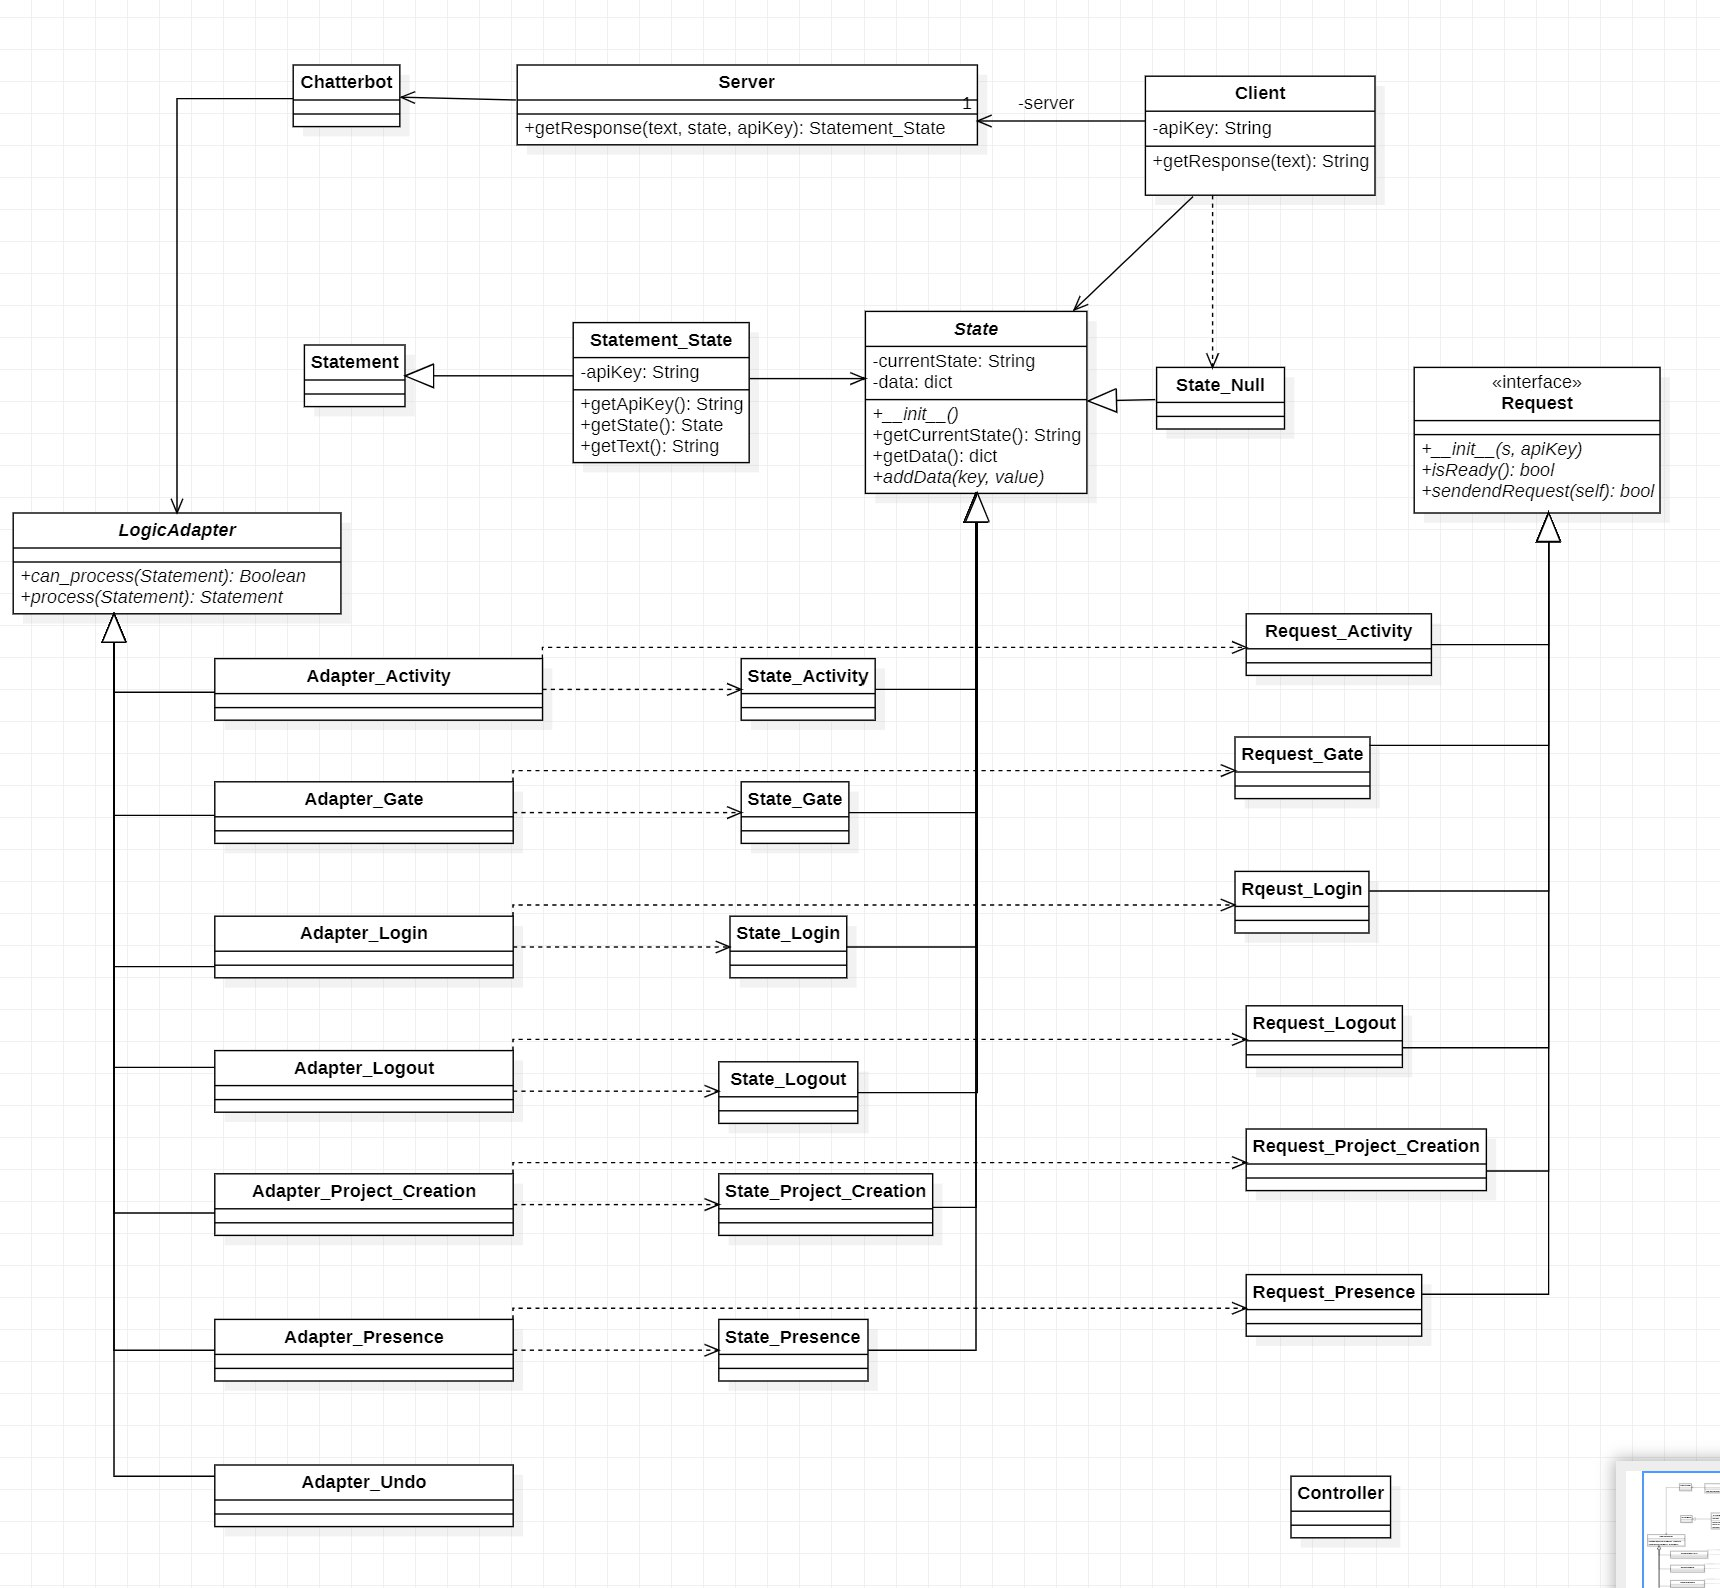
\includegraphics[scale=0.70]{images/diagramma_classi.jpg}
    \caption{Diagramma UML delle classi lato Server}
	\end{figure}

\newpage

\subsection{Server}
\subsubsection{App} Unico punto dell'applicativo dove viene interfacciato l'utente, qui viene istanziato il server e la lista dei client. Inoltre viene definito il routing delle richieste del client grazie al framework Flask. 
\subsubsection{Client} Classe che rappresenta ogni client connesso. Quando viene istanziata mantiene lo stato interno della richiesta, e con il metodo getResponse trasmette la richiesta al server.
\subsubsection{Server} Classe che inizializza la libreria esterna \textit{Chatterbot}. Presenta il metodo getResponse, il quale crea lo \textit{Statement\_State} con i parametri forniti dal Client e scorre tutti gli adapter cercando di rispondere in modo corretto alla richiesta. 
\subsubsection{Chatterbot} Classe della libreria esterna \glossario{Chatterbot}. Rappresenta un istanza del ChatBot e tutti gli adapter ad esso collegati.
\subsubsection{Statement} Classe della libreria esterna \glossario{Chatterbot}. Rapprensenta un input che il ChatBot riceve o un output che il ChatBot ritorna in merito all'input ricevuto.
\subsubsection{LogicAdapter} Classe della libreria esterna \glossario{Chatterbot}. Determina la logica di come il ChatterBot seleziona la risposta allo Statement di input. I suoi due metodi can\_process e process sono il fulcro dell'applicativo lato server. can\_process determina se una richiesta può essere soddisfatta dall'adapter, process definisce come elaborarla. Questa classe viene usata come classe base astratta per tutti gli adapter, questi infatti ereditano da LogicAdapter i due metodi e li sovvrascrivono per creare la propria logica di risposta.
\subsubsection{State} Interfaccia che definisce il contratto di tutti i vari stati. Presenta i tre metodi che gli stati implementano per assolvere ognuno alla propria funzione. All'interno di ogni State saranno definiti i dati, in forma di dizionario (chiave, valore),  necessari per completare la richiesta e su questi implementati i vari metodi. In generale getCurrentState ritornerà lo stato corrente, getData ritornerà i dati definiti all'interno di ogni State e addData aggiungerà un dato al dizionario.
\paragraph*{State\_Null} Implementa l'interfaccia \textit{State}, di particolare importanza perchè non è associato a nessun adapter. Serve per simulare lo stato nullo, viene utilizzato quando l'utente non è in nessun'altro stato.
\subsubsection{Statement\_State} Sottoclasse di Statement (classe della libreria esterna \glossario{Chatterbot}). Estende lo Statement di Chatterbot con lo State e l'ApiKey della richiesta. 
\subsubsection{Request} Interfaccia che definisce tutte le request. Presenta due metodi isReady e sendRequest il quale funzionamento verrà implementato per ogni request. In generale isReady verifica se la request è pronta per essere inviata, mentre invece sendRequest invia la richiesta \glossario{HTTP} alle \glossario{API Rest} di Imola Informatica per interagire con i loro servizi, e ritorna una risposta per verificare se la richiesta è andata a buon fine o meno.
\subsubsection{Login} Classi \textit{Adapter\_Login}, \textit{State\_Login} permettono di effettuare il login
\subsubsection{Logout} Classe \textit{Adapter\_Logout} permette di effettuare il logout.
\subsubsection{Activity} Classi \textit{Adapter\_Activity}, \textit{State\_Activity} e \textit{Request\_Activity}. Sono le classi necessarie per comporre ed inviare una richiesta di consuntivazione per un attività svolta su un progetto esistente. La richiesta viene composta con i campi codice progetto, data , ore fatturabili, ore viaggio, ore viaggio fatturabili, sede, fatturabile (campo che determina se è fatturabile o meno) e descrizione.
\subsubsection{Gate} Classi \textit{Adapter\_Gate}, \textit{State\_Gate} e \textit{Request\_Gate}. Sono le classi necesssarie a comporre ed inviare una richiesta per l'apertura del cancello. La richiesta viene composta con il campo sede che determina la sede della quale aprire il cancello.
\subsubsection{Project\_Creation} Classi \textit{Adapter\_Project\_Creation}, \textit{State\_Project\_Creation} e \textit{Request\_Project\_Creation}. Sono le classi necessarie per comporre ed inviare una richiesta per la creazione di un nuovo progetto. La richiesta è composta dai campi codice progetto, dettagli, cliente, manager, status (che viene di default inizializzato come iniziale), area, data inizio, data fine.
\subsubsection{Presence} Classi \textit{Adapter\_Presence}, \textit{State\_Presence} e \textit{Request\_Presence}. Sono le classi necessarie per comporre ed inviare la richiesta di registrazione in presenza presso una sede. La richiesta è composta dall'unico campo sede che determina appunto la sede nella quale si vuole registrare la presenza.
\subsubsection{Get Activity} Classi \textit{Adapter\_Get\_Activity}, \textit{State\_Get\_Activity} e \textit{Request\_Get\_Activity}. Sono le classi necessarie a comporre la richiesta per visualizzare le consuntivazioni già effettuate per un progetto esistente. L'unico campo che compone la richiesta è il codice progetto per il quale si vuole visualizzare tutto quello che fin'ora è stato consuntivato.
\subsubsection{Undo} Classe \textit{Adapter\_Undo}. Permette di annullare qualsiasi operazione in corso e inserire la richiesta per la stessa o un'altra funzionalità.
\subsection{Diagramma di sequenza Esecuzione Richiesta}
\newpage

\begin{landscape}
	\begin{figure}[H]
	\centering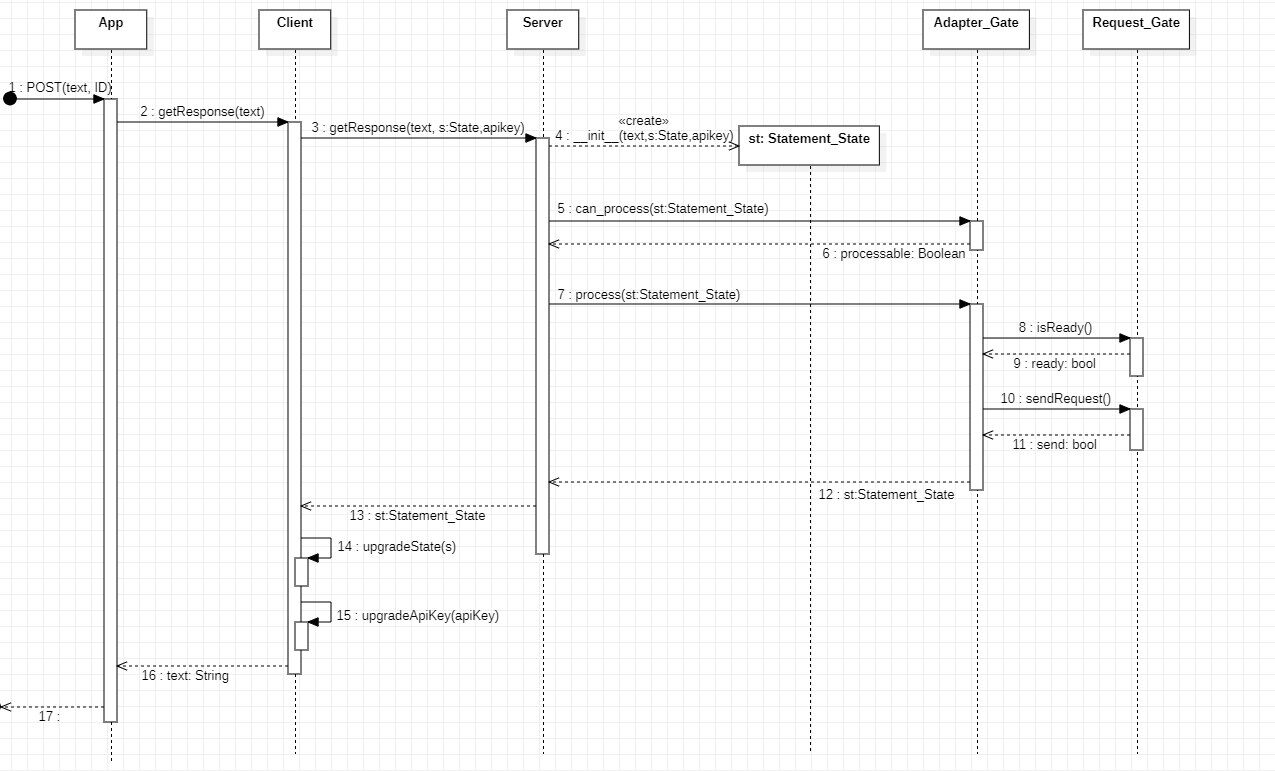
\includegraphics[width=\linewidth]{images/diagramma_sequenza_server.jpg}
    \caption{Diagramma di sequenza Esecuzione Richiesta }
	\end{figure}
\end{landscape}
\begin{itemize}
    \item Il \glossario{Client} web effettua una richiesta POST all'\textit{App}, che si compone di testo inserito dall'utente (text) e identificativo univoco del \textit{Client} connesso (ID).
    \item \textit{App} riceve la richiesta, seleziona il corretto \textit{Client} che deve gestirla mediante l'ID ricevuto e inoltra a \textit{Client} il testo della richiesta invocando il metodo \textit{getResponse}.
    \item Il \textit{Client} richiama il metodo del \textit{Server} \textit{getResponse} passandogli il testo della richiesta, lo stato attuale della richiesta e l'\textit{ApiKey} con la quale la richiesta è stata effettuata.
    \item Il \textit{Server} riceve la richiesta del \textit{Client}, crea lo \textit{Statement\_State} con i tre dati che ha ricevuto, e invoca la libreria Chatterbot per cercare la risposta più pertinente al testo della richiesta (in questo caso "apertura cancello"). In questo caso il Server fa la richiesta ad \textit{Adapter\_Gate} con il metodo \textit{can\_process}, passando come paramentro lo \textit{Statement\_State} che ha creato.
    \item \textit{Adapter\_Gate} risponde con un boolean alla richiesta per determinare se può processarla o meno, e lo ritorna al \textit{Server}.
    \item Il server richiama \textit{Adapter\_Gate} per processare la richiesta passando come parametro lo \textit{Statement\_State} che ha creato.
    \item \textit{Adapter\_Gate} prepara la richiesta, in base ai dati che ha ricevuto e verifica con il metodo \textit{isReady} di \textit{Request\_Gate} se questa è pronta per essere effettuata. \textit{Request\_Gate} risponde con un boolean indicando se la richiesta è pronta o meno per essere eseguita.
    \item Se la richiesta è pronta per essere effettuata (come nell'esempio) \textit{Adapter\_Gate} invoca il metodo \textit{sendRequest} di \textit{Request\_Gate} per effettuare realmente la richiesta verso le API di Imola Informatica. \textit{Request\_Gate} riponde con un boolean che indica se la richiesta è andata a buon fine.
    \item A questo punto \textit{Adapter\_Gate} ritorna lo \textit{Statement\_State} al server che aveva iniziato la richiesta con il metodo \textit{process}.
    \item Il \textit{Server} dopo aver ricevuto lo \textit{Statement\_State} in risposta dell'adapter lo trasmette al \textit{Client} che aveva fatto la richiesta \textit{getResponse}.
    \item Il \textit{Client} riceve lo \textit{Statement\_State}, aggiorna il proprio stato con il metodo \textit{upgradeState} e la propria \textit{ApiKey} con il metodo \textit{upgradeApiKey}. Infine ritorna ad \textit{App} la risposta sotto forma di string (text) perchè venga indirizzata al \glossario{Client} web.
\end{itemize}
\subsection{Diagramma di sequenza Richiesta Identificativo}
\begin{figure}[H]
    \centering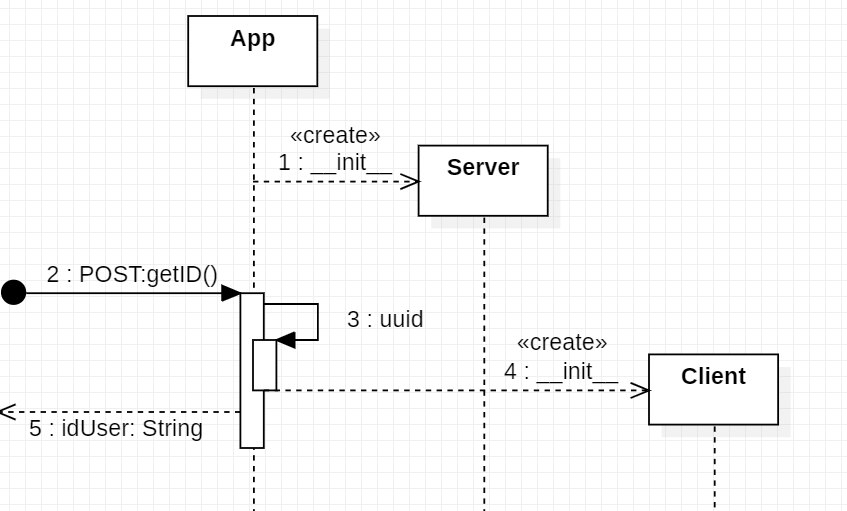
\includegraphics[width=\linewidth]{images/diagramma_sequenza_client.jpg}
    \caption{Diagramma di sequenza Richiesta Identificativo}
\end{figure}
\begin{itemize}
    \item Il \glossario{Client} web effettua una richiesta POST \textit{getID} ad \textit{App} richiedendo un ID.
    \item \textit{App} riceve la richiesta del nuovo Client che vuole connettersi al \textit{Server}, precedentemente creato e inizializzato, e crea un \glossario{UUID}, per identificarlo univocamente in tutte le comunicazioni.
    \item \textit{App} in seguito crea ed inizializza un \textit{Client} nuovo associato al ID appena creato.
    \item Infine \textit{App} ritorna al \glossario{Client} web l'identificativo univoco creato sotto forma di un campo stringa (idUser).
\end{itemize}
\newpage

\subsection{Design Pattern}
Front Controller pattern è un pattern architetturale per la progettazione di applicazioni web che forniscono un punto di ingresso centralizzato per la gestione delle richieste. Nel caso del nostro applicativo infatti la classe \textit{App}, in cui è presente \glossario{Flask} si occupa di ricevere tutte le richieste ricevute dai vari \glossario{Client}, le quali verranno poi gestite da un'istanza della classe \textit{Client} lato \glossario{Server} che andrà a contattare l'adapter corretto in base all'interpretazione del messaggio, effettuando in seguito una chiamata all'API-REST consona al servizio richiesto.
\newpage

\subsection{API Rest Imola Informatica} L'azienda ha fornito delle \glossario{API Rest} che permettono al \glossario{chatbot} di interagire con i loro sistemi aziendali. Sono facilmente consultabili a questo \href{https://apibot4me.imolinfo.it/}{\color{blue} link}.
\subsubsection{Consuntivazione di un attività}
\paragraph{API Url} \hfill \break
/projects/\{code\}/activities/me
\paragraph{Metodo di richiesta \glossario{HTTP}} \hfill \break
POST
\paragraph{Headers \glossario{HTTP}}
\begin{itemize}
    \item \textbf{accept}: application/json;
    \item \textbf{api\_key}: api\_key, per autorizzare le richieste;
    \item \textbf{Content-Type}: application/json.
\end{itemize}
\paragraph{Parametri URL} \hfill \break
\begin{center}
    \renewcommand{\arraystretch}{1.8}
    \begin{tabular}{ |m{10em}|m{4em}|m{20em}| }
        \hline
        \textbf{Nome} & \textbf{Tipo} & \textbf{Descrizione} \\
        \hline
        code & string & rappresenta il codice del progetto di cui fa parte l’attività da rendicontare.\\
        \hline
    \end{tabular}
\end{center}
\paragraph{Parametri Body} \hfill \break
Nel body della richiesta viene passato un array contenente un json con questi parametri
\begin{center}
    \renewcommand{\arraystretch}{1.8}
    \begin{tabular}{ |m{10em}|m{4em}|m{20em}| }
        \hline
        \textbf{Nome} & \textbf{Tipo} & \textbf{Descrizione} \\
        \hline
        date & string & data in cui si è svolta l'attività.\\
        \hline
        billableHours & int & ore fatturabili dell'attività.\\
        \hline
        travelHours & int & ore di viaggio spese per l'attività.\\
        \hline
        billableTravelHours & int & ore di viaggio fatturabili per l'attività.\\
        \hline
        location & string & nome della sede in cui si è svolta l'attività.\\
        \hline
        billable & bool & indica se l'attività è fatturabile.\\
        \hline
        note & string & descrizione dell'attività.\\
        \hline
    \end{tabular}
\end{center}
\paragraph{Risposte}
\begin{center}
    \renewcommand{\arraystretch}{1.8}
    \begin{tabular}{ |m{9em}|m{24em}| }
        \hline
        \textbf{Status code \glossario{HTTP}} & \textbf{Descrizione} \\
        \hline
        204 & indica che la richiesta di consuntivazione è andata a buon fine\\
        \hline
        404 & indica che il codice specificato del progetto non è corretto\\
        \hline
        401 & indica che l'api key non è stata specificata o quella utilizzata non è valida.\\
        \hline
    \end{tabular}
\end{center}
\subsubsection{Apertura del cancello}
\paragraph{API Url} \hfill \break
/locations/\{location\_name\}/devices/\{device\}/status
\paragraph{Metodo di richiesta \glossario{HTTP}} \hfill \break
PUT
\paragraph{Headers \glossario{HTTP}}
\begin{itemize}
    \item \textbf{accept}: application/json;
    \item \textbf{api\_key}: api\_key, per autorizzare le richieste;
    \item \textbf{Content-Type}: application/json.
\end{itemize}
\paragraph{Parametri URL} \hfill \break
\begin{center}
    \renewcommand{\arraystretch}{1.8}
    \begin{tabular}{ |m{10em}|m{4em}|m{20em}| }
        \hline
        \textbf{Nome} & \textbf{Tipo} & \textbf{Descrizione} \\
        \hline
        location\_name & string & sede di cui aprire il cancello.\\
        \hline
        device & string & nome del dispositivo da utilizzare, in questo caso il cancello.\\
        \hline
    \end{tabular}
\end{center}
\paragraph{Parametri Body} \hfill \break
Nel body della richiesta viene passato un json contenente questi parametri
\begin{center}
    \renewcommand{\arraystretch}{1.8}
    \begin{tabular}{ |m{10em}|m{4em}|m{20em}| }
        \hline
        \textbf{Nome} & \textbf{Tipo} & \textbf{Descrizione} \\
        \hline
        status & string & rappresenta il nuovo stato del dispositivo.\\
        \hline
    \end{tabular}
\end{center}
\paragraph{Risposte}
\begin{center}
    \renewcommand{\arraystretch}{1.8}
    \begin{tabular}{ |m{9em}|m{24em}| }
        \hline
        \textbf{Status code \glossario{HTTP}} & \textbf{Descrizione} \\
        \hline
        204 & indica che la richiesta di apertura del cancello è andata a buon fine.\\
        \hline
        404 & indica che la sede di cui aprire il cancello non è valida.\\
        \hline
        401 & indica che l'api key non è stata specificata o quella utilizzata non è valida.\\
        \hline
    \end{tabular}
\end{center}
\subsubsection{Registrazione della presenza}
\paragraph{API Url} \hfill \break
/locations/\{location\_name\}/presence
\paragraph{Metodo di richiesta \glossario{HTTP}} \hfill \break
POST
\paragraph{Headers \glossario{HTTP}}
\begin{itemize}
    \item \textbf{accept}: application/json;
    \item \textbf{api\_key}: api\_key, per autorizzare le richieste;
    \item \textbf{Content-Type}: application/json.
\end{itemize}
\paragraph{Parametri URL} \hfill \break
\begin{center}
    \renewcommand{\arraystretch}{1.8}
    \begin{tabular}{ |m{10em}|m{4em}|m{20em}| }
        \hline
        \textbf{Nome} & \textbf{Tipo} & \textbf{Descrizione} \\
        \hline
        location\_name & string & sede in cui registrare la presenza.\\
        \hline
    \end{tabular}
\end{center}
\paragraph{Risposte}
\begin{center}
    \renewcommand{\arraystretch}{1.8}
    \begin{tabular}{ |m{9em}|m{24em}| }
        \hline
        \textbf{Status code \glossario{HTTP}} & \textbf{Descrizione} \\
        \hline
        200 & indica che la registrazione della presenza è stata effettuata con successo.\\
        \hline
        404 & indica che la sede specificata non è valida.\\
        \hline
        401 & indica che l'api key non è stata specificata o quella utilizzata non è valida.\\
        \hline
    \end{tabular}
\end{center}
\subsubsection{Creazione di un nuovo progetto}
\paragraph{API Url} \hfill \break
/projects
\paragraph{Metodo di richiesta \glossario{HTTP}} \hfill \break
POST
\paragraph{Headers \glossario{HTTP}}
\begin{itemize}
    \item \textbf{accept}: application/json;
    \item \textbf{api\_key}: api\_key, per autorizzare le richieste;
\end{itemize}
\paragraph{Parametri Body} \hfill \break
Nel body della richiesta viene passato un json contenente questi parametri
\begin{center}
    \renewcommand{\arraystretch}{1.8}
    \begin{tabular}{ |m{10em}|m{4em}|m{20em}| }
        \hline
        \textbf{Nome} & \textbf{Tipo} & \textbf{Descrizione} \\
        \hline
        code & string & codice del progetto da creare.\\
        \hline
        detail & string & descrizione del progetto da creare.\\
        \hline
        customer & string & cliente per cui viene creato il progetto.\\
        \hline
        manager & string & manager del progetto da creare.\\
        \hline
        status & string & stato del progetto.\\
        \hline
        area & string & sede in cui svolgere il progetto.\\
        \hline
        startDate & string & data di inizio del progetto.\\
        \hline
        endDate & string & data di fine del progetto.\\
        \hline
    \end{tabular}
\end{center}
\paragraph{Risposte}
\begin{center}
    \renewcommand{\arraystretch}{1.8}
    \begin{tabular}{ |m{9em}|m{24em}| }
        \hline
        \textbf{Status code \glossario{HTTP}} & \textbf{Descrizione} \\
        \hline
        204 & indica che è l'operazione di creazione del progetto è andata a buon fine.\\
        \hline
        400 & indica che almeno uno dei parametri non è stato specificato.\\
        \hline
        401 & indica che l'api key non è stata specificata o quella utilizzata non è valida.\\
        \hline
    \end{tabular}
\end{center}
\subsubsection{Recupero delle sedi}
\paragraph{API Url} \hfill \break
/locations
\paragraph{Metodo di richiesta \glossario{HTTP}} \hfill \break
GET
\paragraph{Headers \glossario{HTTP}}
\begin{itemize}
    \item \textbf{accept}: application/json;
    \item \textbf{api\_key}: api\_key, per autorizzare le richieste;
\end{itemize}
\paragraph{Risposte}
\begin{center}
    \renewcommand{\arraystretch}{1.8}
    \begin{tabular}{ |m{9em}|m{24em}| }
        \hline
        \textbf{Status code \glossario{HTTP}} & \textbf{Descrizione} \\
        \hline
        200 & ritorna una lista contenente le informazioni delle sedi.\\
        \hline
        401 & indica che l'api key non è stata specificata o quella utilizzata non è valida.\\
        \hline
    \end{tabular}
\end{center}
\subsubsection{Recupero della rendicontazione per il progetto corrente}
\paragraph{API Url} \hfill \break
/projects/\{code\}
\paragraph{Metodo di richiesta \glossario{HTTP}} \hfill \break
GET
\paragraph{Headers \glossario{HTTP}}
\begin{itemize}
    \item \textbf{accept}: application/json;
    \item \textbf{api\_key}: api\_key, per autorizzare le richieste;
\end{itemize}
\paragraph{Parametri URL} \hfill \break
\begin{center}
    \renewcommand{\arraystretch}{1.8}
    \begin{tabular}{ |m{10em}|m{4em}|m{20em}| }
        \hline
        \textbf{Nome} & \textbf{Tipo} & \textbf{Descrizione} \\
        \hline
        code & string & codice del progetto corrente.\\
        \hline
    \end{tabular}
\end{center}
\paragraph{Risposte}
\begin{center}
    \renewcommand{\arraystretch}{1.8}
    \begin{tabular}{ |m{9em}|m{24em}| }
        \hline
        \textbf{Status code \glossario{HTTP}} & \textbf{Descrizione} \\
        \hline
        200 & ritorna un json contenente le informazioni per il progetto corrente.\\
        \hline
        401 & indica che l'api key non è stata specificata o quella utilizzata non è valida.\\
        \hline
    \end{tabular}
\end{center}

